\documentclass[a4paper,12pt]{article}
\usepackage{style_report} %See style_report.sty for detailed packages


\addbibresource{references_report.bib}

%header and page nrs
\pagestyle{fancy}
\setlength{\headheight}{15pt}
\fancyhf{}
\fancyhead[R]{\rightmark}
\renewcommand{\headrulewidth}{0.4pt}
\renewcommand{\sectionmark}[1]{\markright{#1}}
\fancyfoot[C]{\thepage}  


%titlepage
\begin{document}
	\begin{titlepage}
		\centering
		\begin{figure}[!h]
			\centering
			
\includegraphics[width=0.5\textwidth]{Universität_Zürich_logo.png}
		\end{figure}
		\Large{\textbf{SPI Momentum Strategy \\ Project Paper: Digital Tools for Finance}\\}

		\vfill
		
		\large{Iris Bodenmann\\ Justin Meichtry\\ Maurice Kammermann \\ Steve Nikitas\\}
		
		\vfill
	
		\large{Igor Pozdeev\\Department of Finance\\ University of Zurich\\}

        \vfill
        \large{December 11th, 2024}
	
		\vfill
		\begin{abstract}
            In this paper, we examine the ability of long-only momentum strategies as proposed by \cite{jegatit1993} to generate excess returns in the Swiss stock market from 2000 to 2024. Our primary focus is on whether this strategy remains profitable to this day, even after accounting for transaction costs - the main drawback of momentum strategies. Our results indicate that long-only momentum strategies in the Swiss market can indeed generate significant abnormal net returns, even after accounting for transaction costs, and consistently outperform the SPI benchmark.  
			
			\vspace{2mm}
			
			\textbf{Keywords:} Momentum, Anomaly, Swiss Stock Market\\
            \textbf{JEL Classification:} G4, G14, G17
		\end{abstract}
		
		
	\end{titlepage}
    
%table of contents
\pagenumbering{roman}
\setcounter{page}{1}
\tableofcontents

\clearpage
\listoftables
\listoffigures
\clearpage


%Introduction
\pagenumbering{arabic}
\setcounter{page}{1}
\section{Introduction}
The momentum effect, a prominent market anomaly first documented by \cite{jegatit1993}, continues to intrigue researchers and challenge the efficient market hypothesis. This study examines the momentum effect in the Swiss stock market, focusing on individual stocks and accounting for transaction costs. Our primary aim is to replicate the work of \cite{jegatit1993} within the Swiss stock market context. We investigate whether the long-only momentum effect persists in Switzerland to this day and to what extent it can generate abnormal returns. Importantly, we address the most significant drawback of momentum strategies: transaction costs, which diminish returns due to frequent portfolio turnover. By doing so, we tackle the practical challenges of implementing such strategies in real-world conditions. 

We proxy the Swiss stock market using the Swiss Performance Index (SPI). Our dataset comprises daily data for all 205 constituents of the SPI from January 2000 to October 2024, obtained from Bloomberg. To account for the risk-free rate, we use the yield of 1-year Swiss government bonds. The dataset has been cleaned to remove unnecessary information and is free from survivorship bias. 

Our methodology involves ranking all constituents of the SPI based on their past performance over a 6-month lookback period to form portfolios of the 20 top-performing stocks. These portfolios are then held for a 6-month period. Please note that the lookback and holding periods can be adjusted within the source code to test different timeframes. To assess the robustness of this momentum strategy, we systematically vary the lookback periods, holding periods, and transaction costs.  

and results. 

This paper is structured into six sections. Section 2 provides a concise literature review on momentum. Section 3 details the data and methodology used in this study. Section 4 presents the main findings. Section 5 conducts robustness checks. Section 6 concludes with a short summary and practical recommendations for implementation.

\newpage

%Literature Review
\section{Literature Review}
The momentum effect, first documented by \cite{jegatit1993}, describes the tendency of assets that have performed well in the recent past to continue outperforming in the near future, and vice versa for poor performers. This so-called "momentum effect" contradicts the weak form of the efficient market hypothesis, which posits that future returns cannot be predicted using historical price data. 

\cite{jegatit1993} show that a strategy of buying stocks with high returns over the past 3 to 12 months and selling those with low returns over the same period generated significant abnormal returns. This finding was subsequently corroborated by numerous studies across different markets and time periods. For instance, \cite{rouwenhorst1998} confirmed the momentum effect in 12 European stock markets from 1978 to 1995. 

Interestingly, research in the 1980s focused on the "reversal effect," which is conceptually opposite to momentum. \cite{debondt1987} found that past losers outperformed past winners over longer horizons of 3 to 5 years. This long-term reversal effect coexists with the medium-term momentum effect, suggesting a complex pattern of return predictability across different time horizons. 

Specifically for the Swiss market, \cite{rouwenhorst1998} included Switzerland in his study of 12 European markets, confirming the presence of the momentum effect. Additionally, \cite{ammann2008} investigated momentum strategies in the Swiss stock market from 1994 to 2007, finding significant momentum profits even after accounting for transaction costs.

\newpage
%Data and Methodology
\section{Data and Methodology}
\subsection{Data}
The Swiss stock market was proxied using the SPI. Daily total return data for the SPI and its 205 constituents were obtained from Refinitiv Datastream, covering the period from 2000 to 2024. The risk-free rate data, represented by the monthly yield of a 1-year Swiss government bond for the same period, were retrieved from the Swiss National Bank (SNB) API. The data set was cleaned for unnecessary information (e.g. currency, empty columns) and constructed to avoid survivorship bias.

\subsection{Methodology}
Our methodology works as follows: We rank the constituents of the SPI based on their past 6-month performance. Equally weighted Portfolios are then formed using the top 20 performing stocks and held for a 6-month period and rebalanced every month. To enhance robustness, we incorporate several variations in our analysis. We test different lookback and holding periods (e.g., 3, 9, and 12 months) to assess the strategy's sensitivity to these parameters. We also simulate various levels of transaction costs to evaluate their impact on performance, acknowledging practical implementation challenges. Additionally, the reader has the ability to adjust all these parameters in the Jupyter Notebook. 



\newpage

%Results
\section{Results}
We examine the performance of long-only and long/short momentum strategies in the Swiss market, evaluating them against the SPI benchmark. To identify general trends, we initially analyze these strategies without factoring in transaction costs.


\begin{table}[htbp]
\centering
\sisetup{
    round-mode=places,
    round-precision=2,
    table-format=2.2
}
\begin{tabular}{lSSS}
\toprule
\multirow{2}{*}{Metric} & \multicolumn{3}{c}{Strategies} \\
\cmidrule(l){2-4}
& {Long-Only} & {Long/Short} & {Benchmark} \\
\midrule
Arithmetic Avg Total Return & 10.8041 & 19.0110 & 2.4043 \\
Arithmetic Avg Excess Return & 8.9813 & 17.1881 & 0.4947 \\
Geometric Avg Total Return & 10.0953 & 18.7608 & 1.4619 \\
Geometric Avg Excess Return & 8.2598 & 16.9252 & -0.4619 \\
Std of Excess Returns (Annualized) & 0.1517 & 0.1835 & 0.1388 \\
Sharpe Ratio (Arithmetic) & 0.5919 & 0.9368 & 0.0356 \\
Sharpe Ratio (Geometric) & 0.5443 & 0.9225 & -0.0333 \\
Min Excess Return & -0.1627 & -0.2214 & -0.1302 \\
Max Excess Return & 0.0990 & 0.1452 & 0.1202 \\
Skewness of Excess Return & -0.7074 & -0.5370 & -0.4670 \\
Kurtosis of Excess Return & 0.9103 & 2.6598 & 0.1039 \\
Alpha (Arithmetic) & 6.0407 & 18.7119 & -0.0000 \\
Alpha (Geometric) & 5.9176 & 18.6500 & 0.0000 \\
T-stat of Alpha & 3.0654 & 5.3641 & -109.7906 \\
Beta (Factor Return) & 0.8642 & -0.4478 & 1.0000 \\
Std Dev of Excess Returns & 0.0438 & 0.0530 & 0.0401 \\
Monthly Excess Return & 0.0075 & 0.0143 & 0.0004 \\
T-stat of Monthly Excess Return & 2.9545 & 4.6762 & 0.1812 \\
Lag 1 Autocorrelation & 0.2153 & 0.1529 & 0.2382 \\
Lag 2 Autocorrelation & 0.1492 & 0.0354 & 0.1383 \\
Lag 3 Autocorrelation & 0.1276 & 0.0499 & 0.1873 \\
\bottomrule
\end{tabular}
\caption{\centering{Summary Statistics Long-Only and Long/Short vs. Benchmark}}
\label{tab_01}
\justifying
\small{Table \ref{tab_01} presents summary statistics pre-transaction costs, for long-only, long/short and the SPI. The rebalanced, equally-weighted momentum portfolios consist of 20 assets each in long/short, based on a 6-month lookback and 6-month holding period.}
\end{table}

The results show that both the long-only and long/short momentum strategies significantly outperform benchmark, achieving greater average total and excess returns, as shown in Table \ref{tab_01}. In comparison to the long-only strategy, the long/short strategy demonstrates superior performance, yielding higher returns with a higher level of risk. 

\begin{figure}[htbp]
\centerline{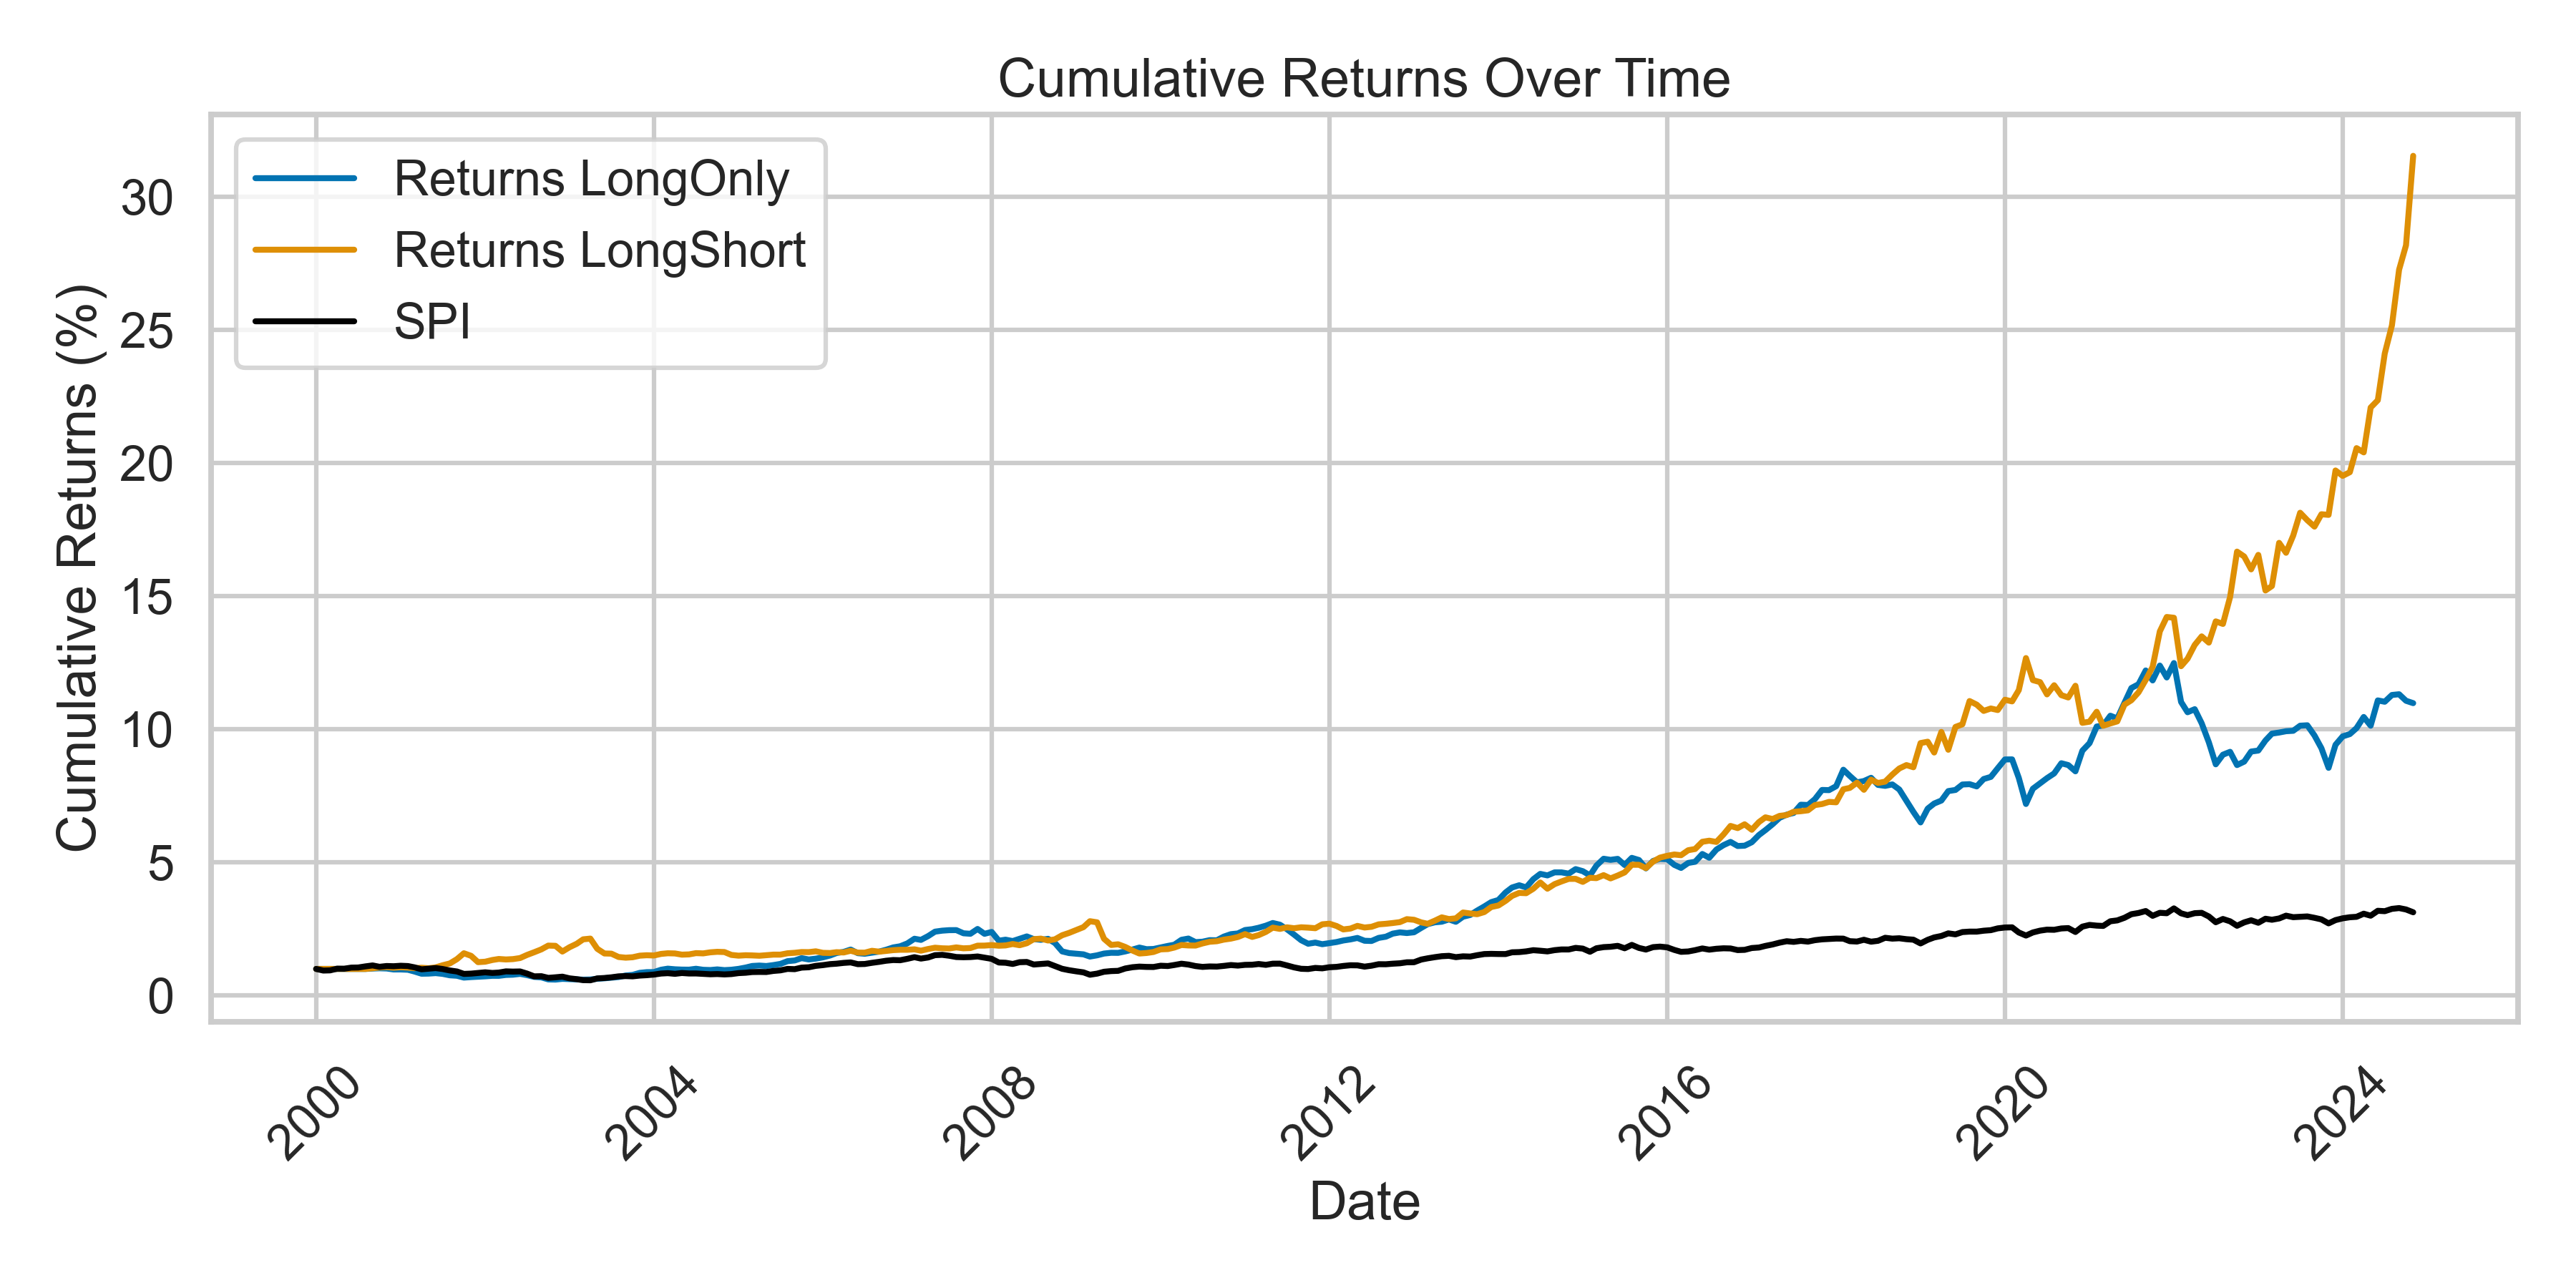
\includegraphics[width=1\textwidth]{figures/cumulative_returns.png}}
\caption{\centering{Cumulative Returns: Long Only Momentum and Long/Short Performance vs. SPI}}
\label{fig_01}
\justifying
\small{{Figure \ref{fig_01} illustrates pre transaction cost cumulative total returns for long-only, long/short and the SPI from January 2000 to October 2024. The rebalanced, equally-weighted momentum portfolios consist of 20 assets each in long/short, based on a 6-month lookback  and 6-month holding period.}}
\end{figure}

Figure \ref{fig_01} illustrates the substantial cumulative outperformance of the long/short strategy relative to both the long-only strategy and the benchmark. Additionally, the performance lines illustrate the moderate correlation between the long-only strategy and the Swiss stock market, as well as the low correlation observed for the long/short strategy.

The outperformance of the long/short momentum strategy is unexpected, especially considering the historical difficulties associated with short components in momentum strategies, which often fail to add value due to returns that fall below the risk-free rate, rendering them unattractive from a risk-return perspective. Contrary to some prior findings, our results indicate that the short component provides value in the Swiss context. We explain this with unique characteristics of the Swiss market, including its low-interest rate environment and relatively low volatility.

Despite the promising performance of the long/short momentum strategy, we will focus on the long-only strategy, as this approach was originally proposed by \cite{jegatit1993}. 

\newpage


%Robustness check
\section{Robustness Check}
While our initial analysis assumed no transaction costs, numerous studies have identified transaction costs as a significant drawback of momentum strategies due to frequent portfolio turnover. To address this crucial aspect and enhance the practical implementation of our long-only strategy, we now explore various parameters that may impact its performance and cost-effectiveness. Specifically, we examine the effects of varying the holding period, lookback period, number of assets held, and transaction costs on the strategy's profitability and feasibility.

Analyzing the relationship between pre-transaction cost Sharpe Ratios and holding periods, we observe a clear negative relationship (see Figure \ref{fig_02}). This finding aligns with \cite{jegatit1993} and the idea that longer holding periods expose momentum portfolios to greater holding period risk, as market conditions or stock-specific factors may shift over time ("reversal of momentum effects"), reducing the effectiveness of the initial momentum signal. 
\begin{figure}[htbp]
\centerline{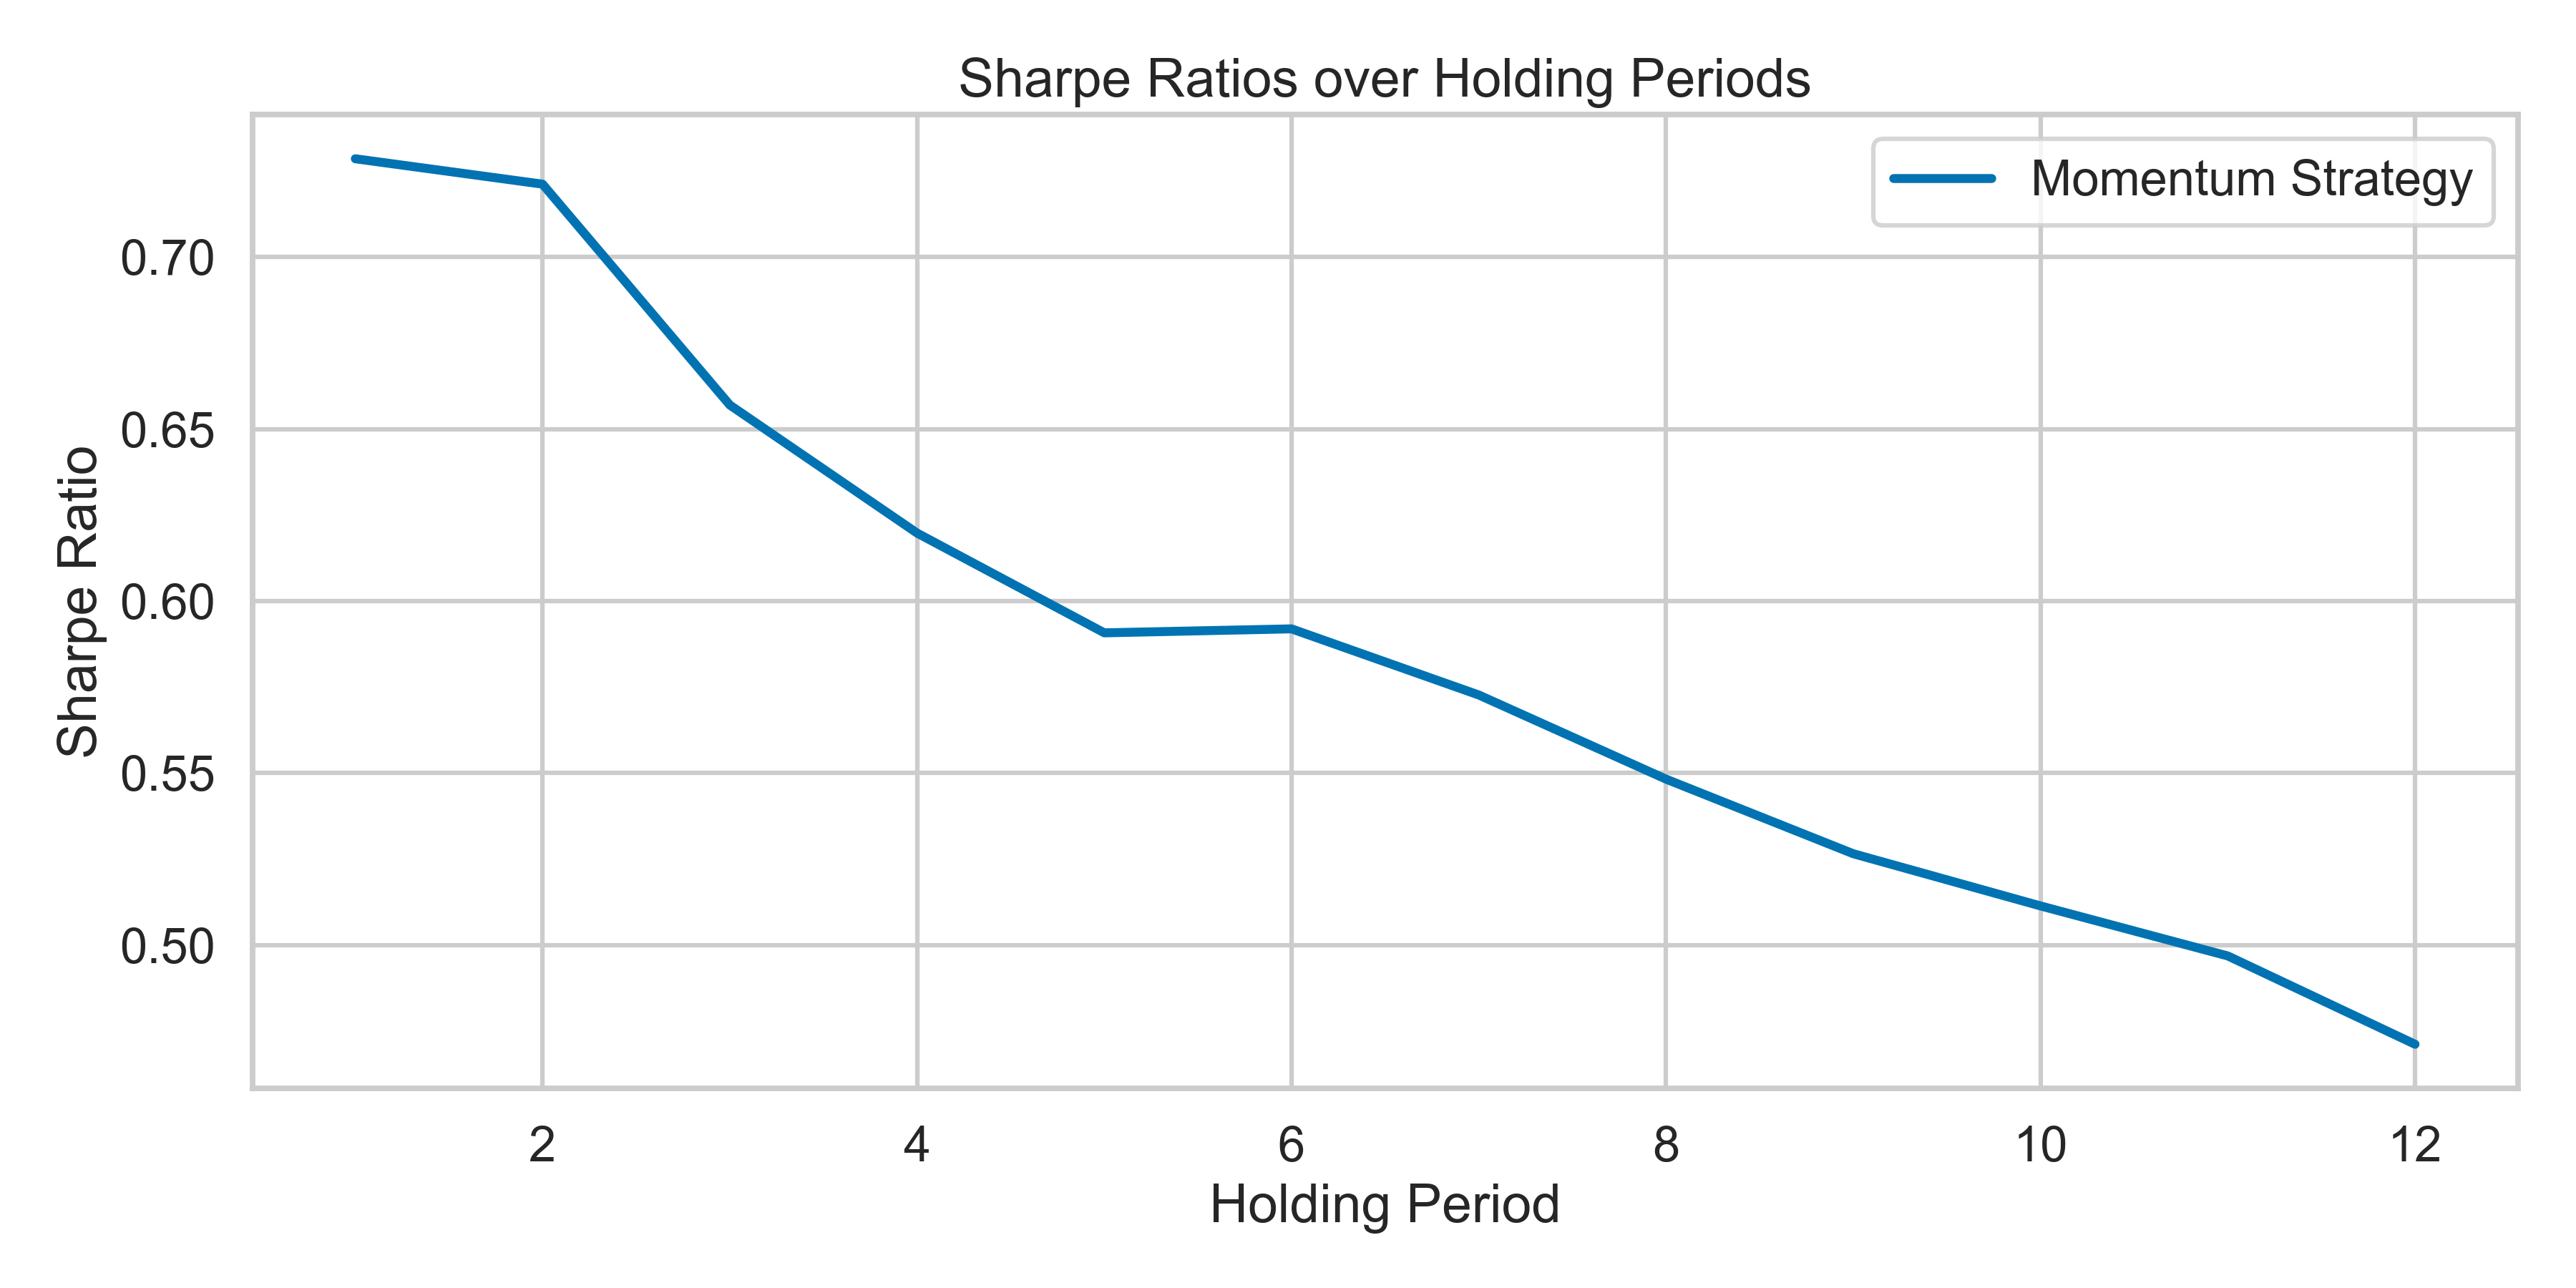
\includegraphics[width=1\textwidth]{figures/rc_holding_period.png}}
\caption{\centering{Sharpe Ratios Over Different Holding Periods}}
\label{fig_02}
\small{{Figure \ref{fig_02} illustrates pre transaction cost Sharpe Ratios for the long-only strategy from January 2000 to October 2024. The rebalanced, equally-weighted momentum portfolios consist of 20 assets, based on a 6-month lookback and varying  holding period (represented on the x-axis).}}
\end{figure}

When analyzing the relationship between pre-transaction cost Sharpe Ratios and lookback periods for the long-only strategy, we find a positive trend that peaks at 10 months before declining (see Figure \ref{fig_03}). This pattern aligns with the idea of \cite{jegatit1993} that intermediate lookback periods effectively capture momentum effects, as they strike a balance between identifying persistent trends and avoiding noise from short-term fluctuations or reversals. The decline beyond 10 months may occur because longer lookback periods incorporate older information that becomes less relevant, diluting the momentum signal.

\begin{figure}[htbp]
\centerline{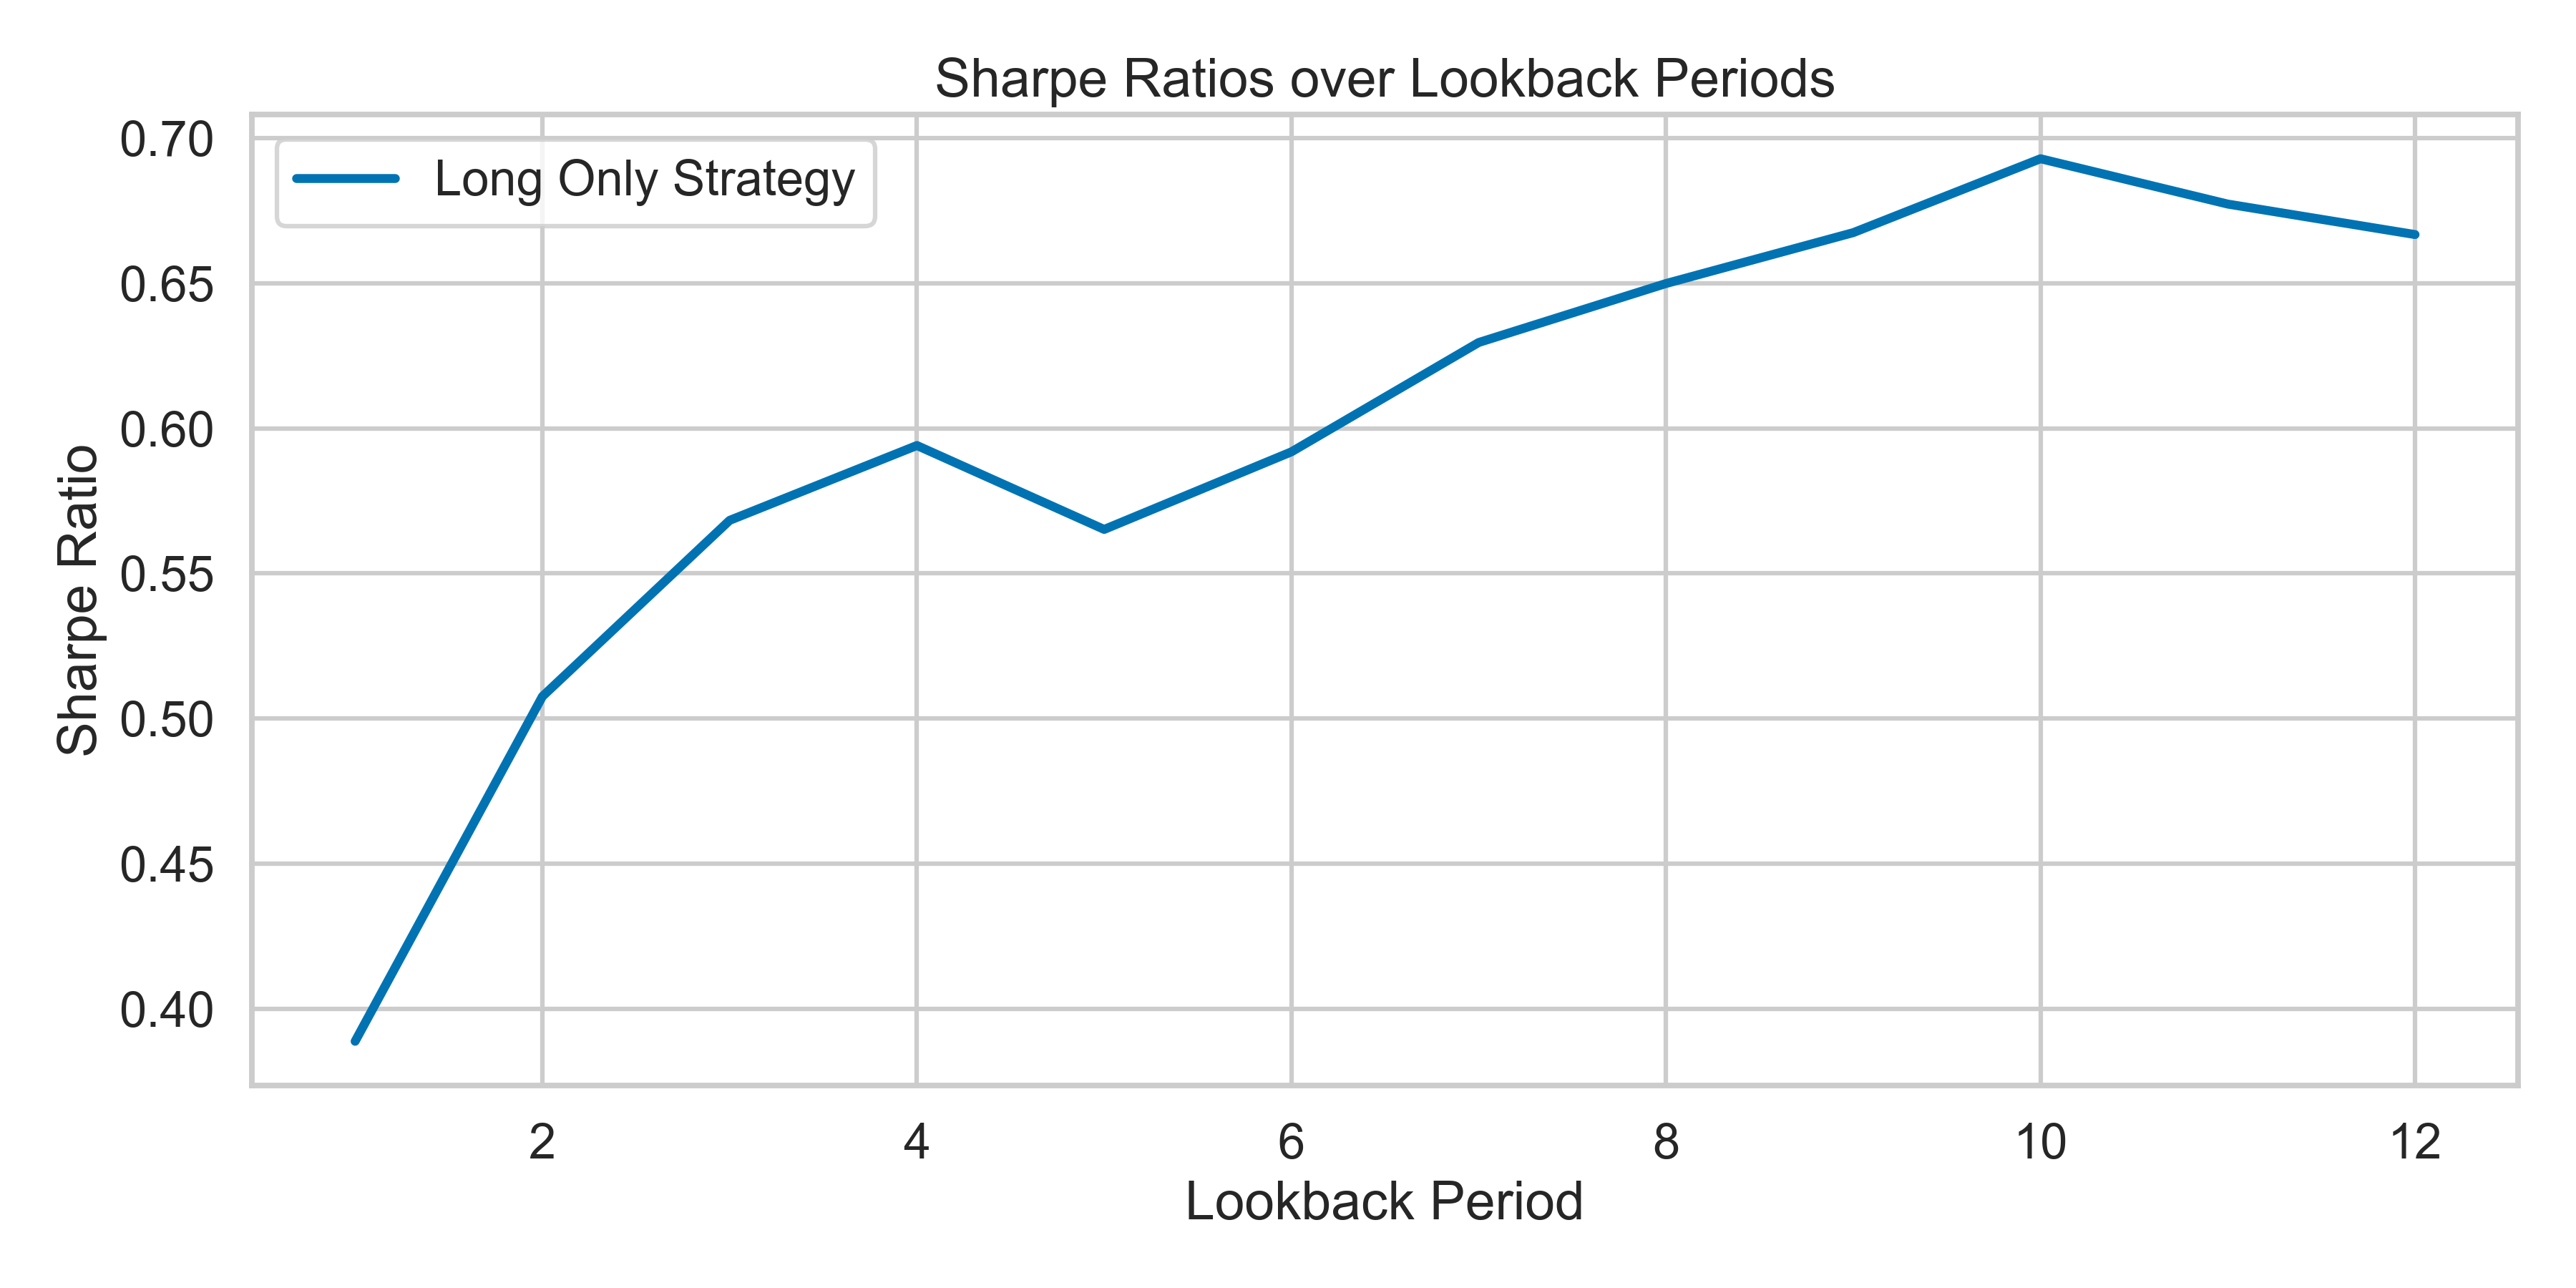
\includegraphics[width=1\textwidth]{figures/rc_lookback_period.png}}
\caption{\centering{Sharpe Ratios Over Different Lookback Periods}}
\label{fig_03}
\small{{Figure \ref{fig_03} illustrates pre transaction cost Sharpe Ratios for the long-only strategy from January 2000 to October 2024. The rebalanced, equally-weighted momentum portfolios consist of 20 assets, based on varying lookback (represented on the x-axis) and 6-month  holding period.}}
\end{figure}

Next, the relationship between pre-transaction cost Sharpe Ratios and number of assets held is examined (see Figure \ref{fig_04}). We observe that the increasing number of holdings improves Sharpe Ratios at the beginning, then, surprisingly, slightly dropping and then increasing. Most likely, this can be explained due to the reduction of volatility because of diversification effects, which diminishes at a certain amount of assets. 
\begin{figure}[htbp]
\centerline{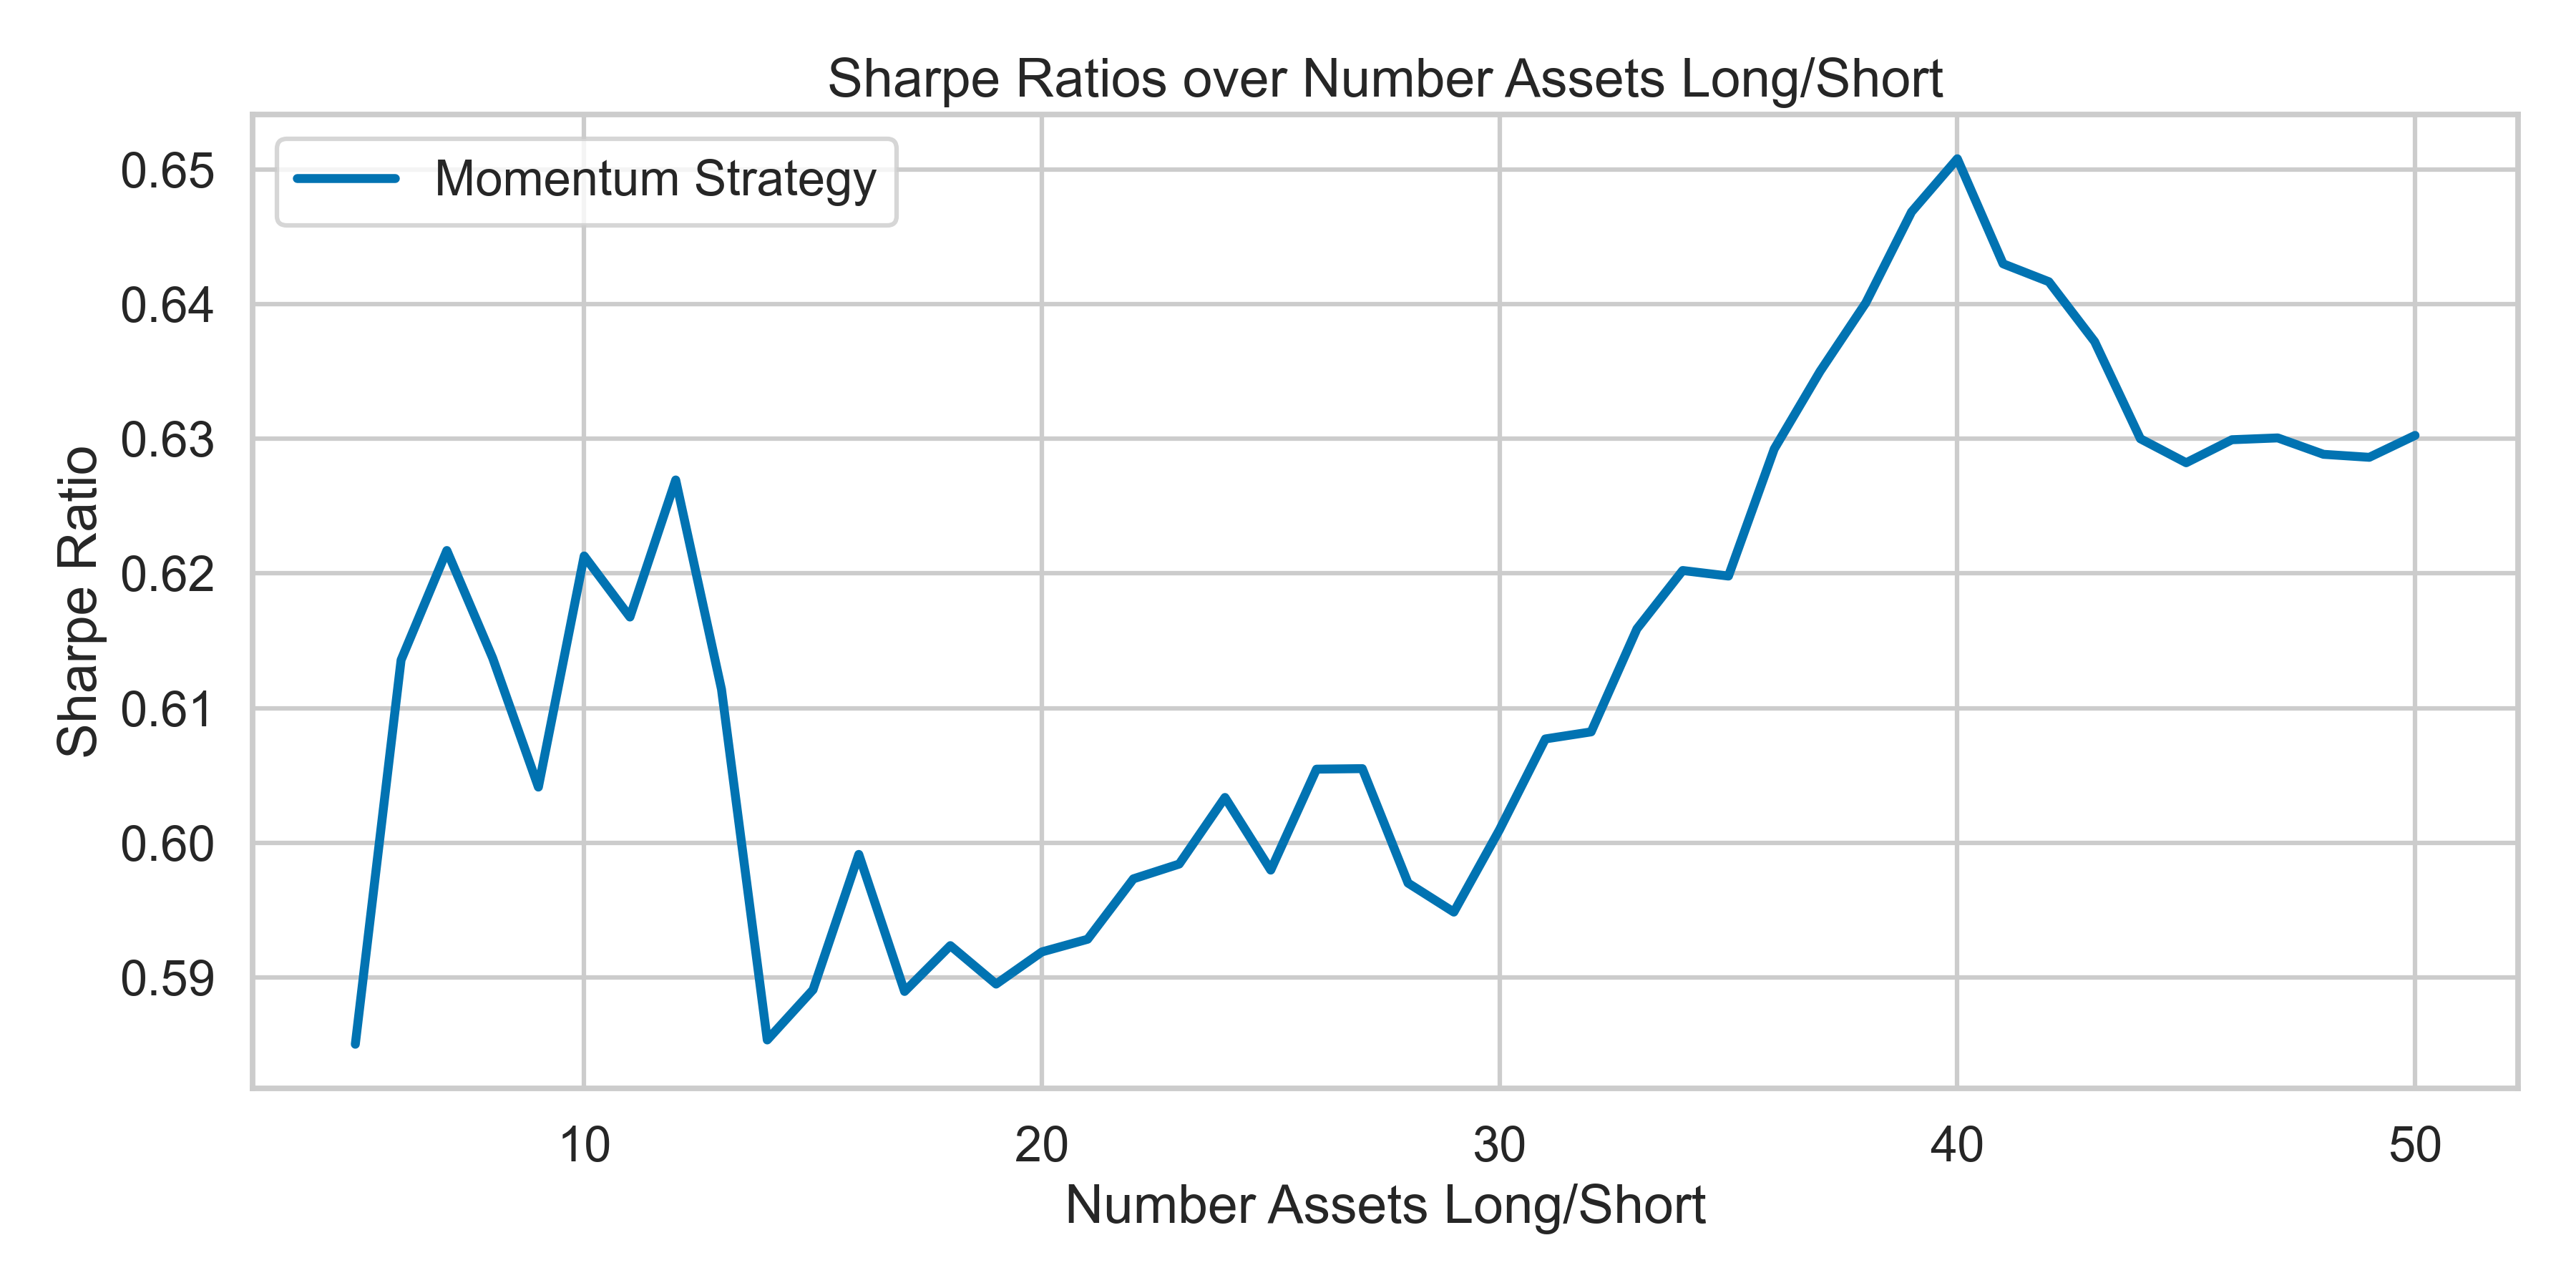
\includegraphics[width=1\textwidth]{figures/rc_number_assets.png}}
\caption{\centering{Sharpe Ratios Over Number of Assets Held}}
\label{fig_04}
\small{{Figure \ref{fig_04} illustrates pre transaction cost Sharpe Ratios for the long-only strategy from January 2000 to October 2024. The rebalanced, equally-weighted momentum portfolios consist of varying amount of assets (represented on the x-axis), based on 6-month lookback and 6-month  holding period.}}
\end{figure}


\begin{figure}[htbp]
\centerline{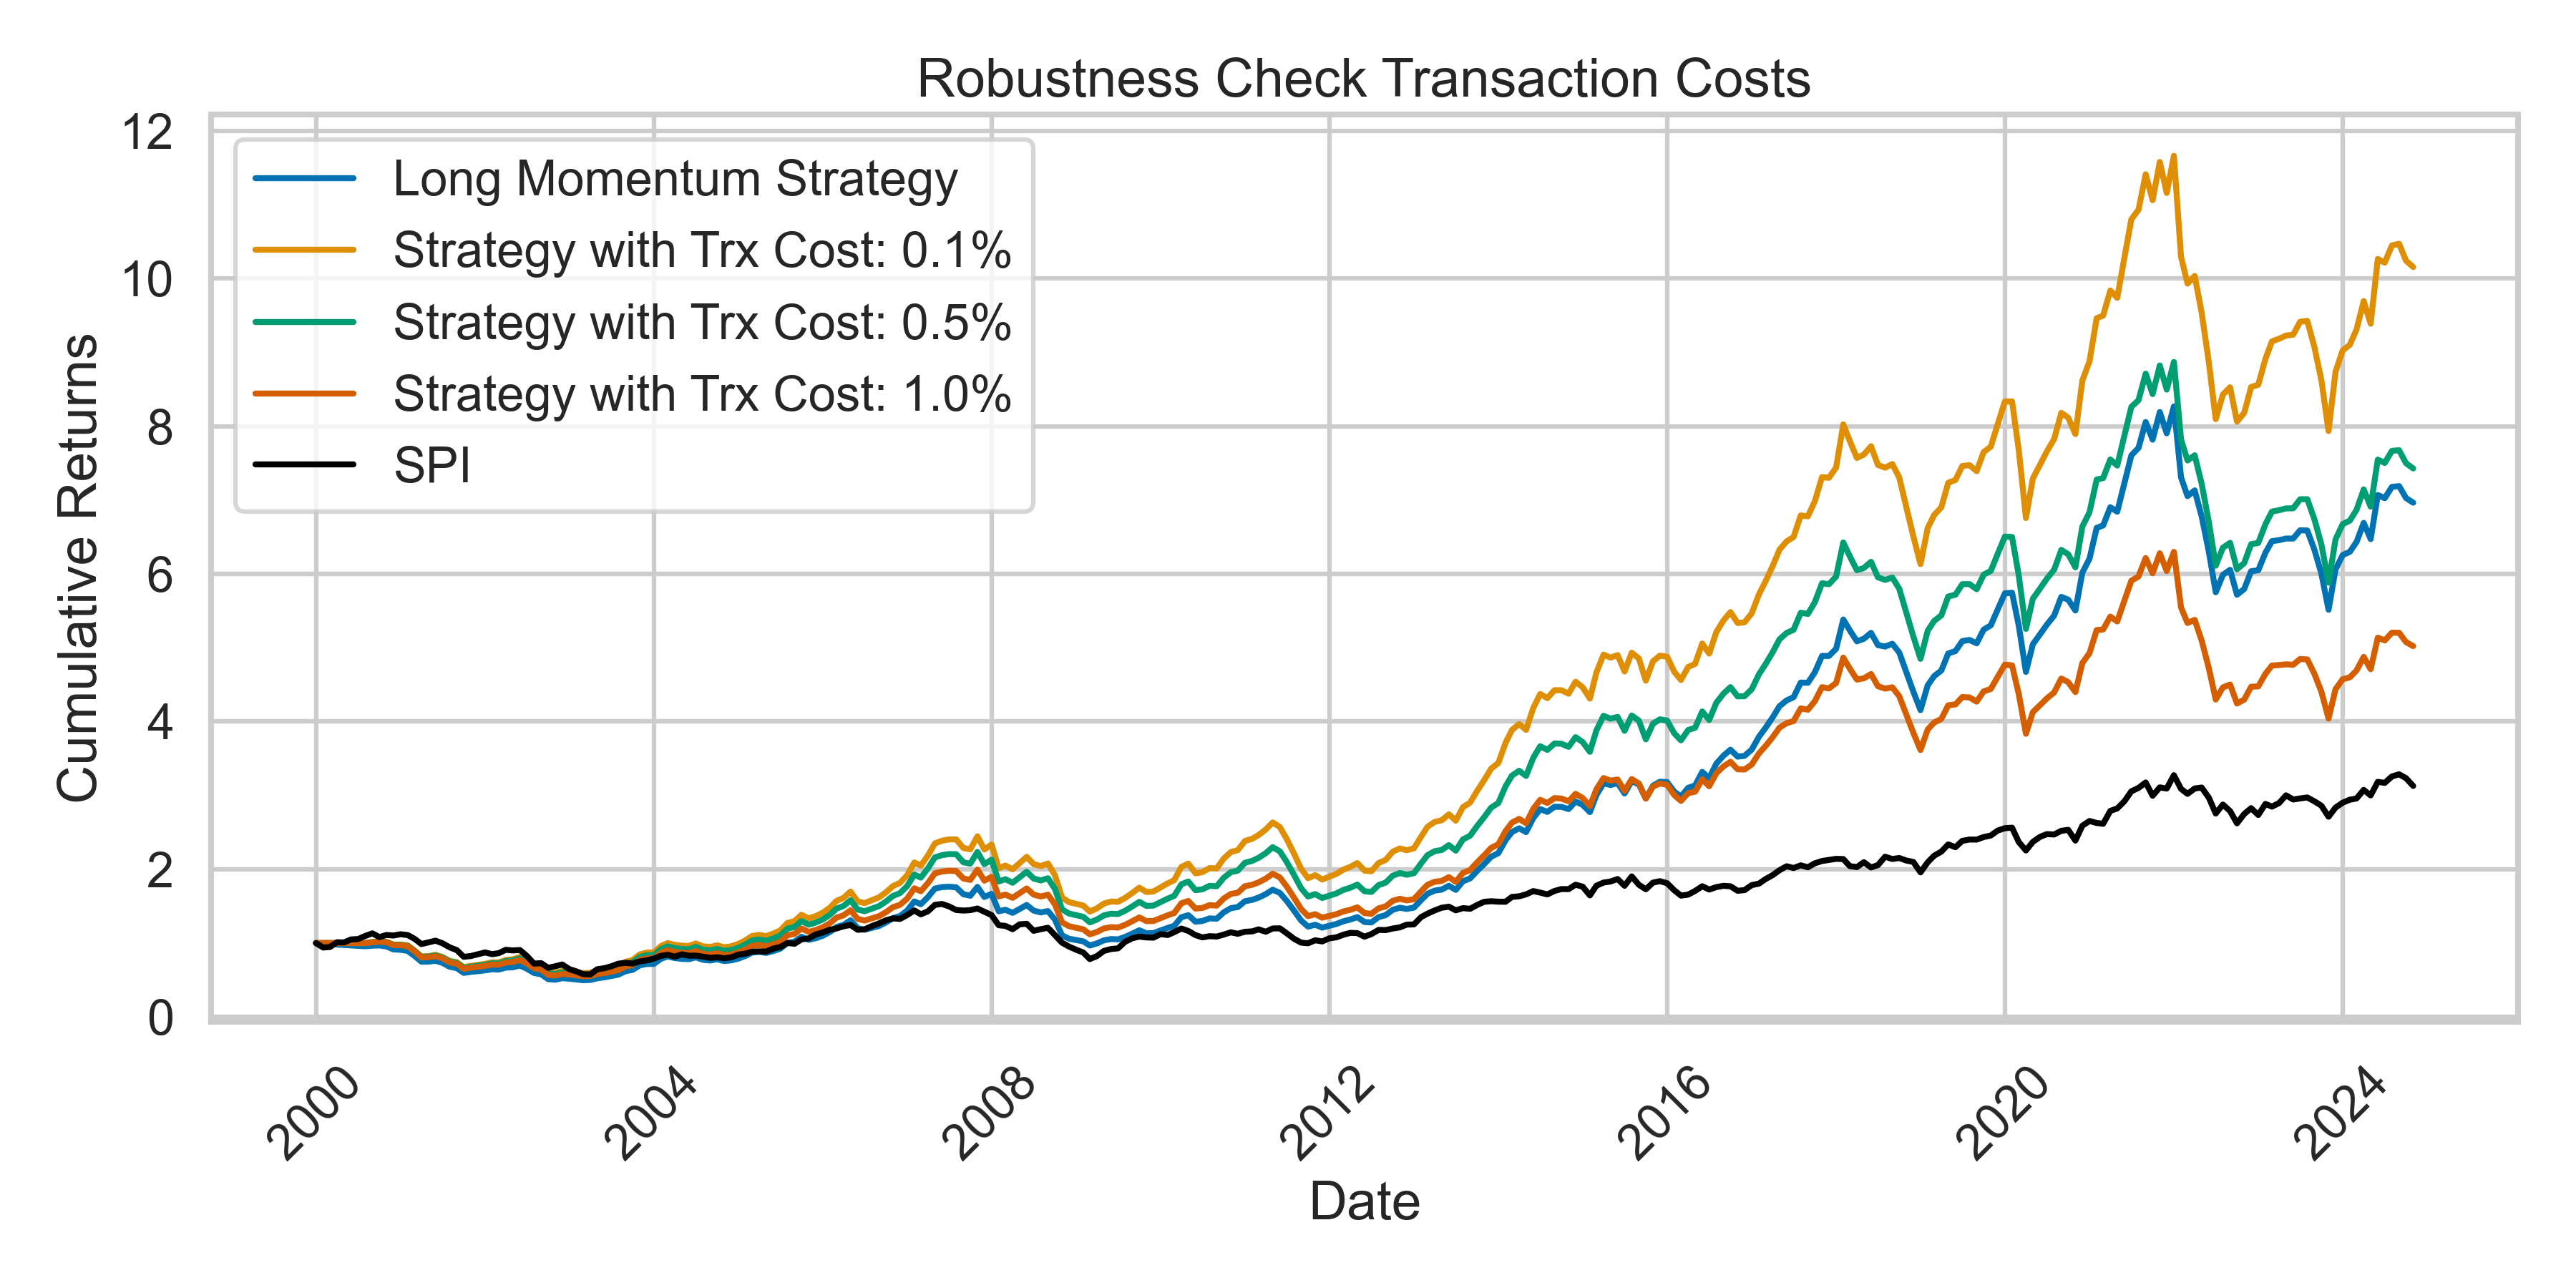
\includegraphics[width=1\textwidth]{figures/rc_trxCost.png}}
\caption{\centering{Net-Cumulative Total Returns Long Only Momentum vs. SPI}}
\label{fig_05}
\small{{Figure \ref{fig_05} illustrates net cumulative total returns for long-only and the SPI from January 2000 to October 2024. The rebalanced, equally-weighted momentum portfolios consist of 20 assets each in long/short, based on a 6-month lookback  and 6-month holding period. Different line colors represent different proportional transactional costs, ranging from 0\% to 1.0\%. No trading cost for SPI applied (buy \& hold).}}
\end{figure}

Lastly, we analyze the impact of varying transaction costs on the profitability of the long-only momentum strategy (see Figure \ref{fig_05}). Despite the well-documented challenges posed by transaction costs in momentum strategies, our findings reveal that the long-only momentum strategy remains highly profitable even with proportional transaction costs of up to 1\%, significantly outperforming the SPI benchmark. However, consistent with previous research, the profitability of these strategies decreases notably with higher transaction costs due to portfolio turnover. 
\newpage

%Conclusion
\section{Conclusion}
Our research investigated the performance and robustness of long-only momentum investment strategies in the Swiss stock market. We analyzed these strategies using the constituents of the Swiss Performance Index (SPI) as our investment universe and examined the robustness of various portfolio parameters such as the holding period, lookback period, the number of holdings, and transaction costs.

Our results confirm that momentum investment strategies can deliver significant excess returns in the Swiss market to this day, consistent with broader academic and empirical evidence. We find that the long-only momentum strategy generates substantial outperformance compared to the SPI benchmark, even after accounting for transaction costs. Despite that, it underperformed relative to the corresponding long/short strategy. Our robustness checks revealed interesting patterns. We observed a negative relationship between holding periods and Sharpe ratios, suggesting shorter holding periods may be more effective. The lookback period analysis showed a peak in performance at around 10 months, aligning with previous research on intermediate lookback periods. Additionally, the strategy demonstrated resilience to transaction costs, remaining profitable even with costs up to 1\%.

In conclusion, we can confidently say that long-only momentum strategies can indeed be  potentially profitable approaches to be implemented in a Swiss market portfolio context. The strategy's resilience to transaction costs and its consistent outperformance of the benchmark suggest its viability for practical application. However, careful consideration must be given to parameters such as holding period, lookback period, and the number of assets held, as these factors can significantly impact the strategy's effectiveness.

Future research could explore the potential benefits of combining this long-only momentum approach with other investment strategies (e.g. value) or extending the analysis to different market conditions and time periods to further test its robustness.

\newpage

%References
\printbibliography


\end{document}
